Neural networks are being deployed in high-stakes applications due to their
state-of-the-art performance for important problems such as image
recognition~\cite{he2016deep}, object detection~\cite{redmon2016you}, and other
perception-related tasks. Among the most famous applications are
self-driving~\cite{grigorescu2020survey}, however they are being studied for
aircraft collision avoidance~\cite{JulianKO18}, drone control~\cite{caps2021}, and
even controllers in medical devices~\cite{tan2021toward}.

While highly performant, neural networks are ``black-boxes.'' Even small neural
networks have thousands of parameters, which makes it impossible for a human to
understand their behavior. In addition, they are notoriously brittle. For
example, they are known to be vulnerable to \textit{adversarial
examples}~\cite{szegedy2013intriguing}, and generally can have undesirable
behaviors~\cite{KatzBDJK17}. This black-box nature combined with their brittleness
raise serious concerns about deploying them in safety-critical systems, where
failures could lead to catastrophe. Indeed, we have already seen catastrophic
failures in self-driving cars, some of which were directly due to failures in deep
learning models~\cite{phil_mccausland_2019}.

This motivates the question: can we ensure that a given neural network behaves
safely? In fact, finding appropriate definitions of safety has proven difficult,
and the main safety property considered by prior work is \textit{robustness},
i.e. proving that semantically meaningless transformations (e.g. adding a small
amount of noise, rotation, scaling, etc.) to a neural network's
input do not cause a change in its output. While important, robustness hardly
covers the entire space of safety properties.

In this dissertation, we focus on safety properties that are
\textit{differential} in nature. Informally, a differential safety property
is a property of two (or more) neural networks or a property of two (or more)
executions of a single network. Various important safety
properties are differential in nature, however, in this dissertation, we focus on
\textit{equivalence} as the canonical differential property. Informally,
proving equivalence means showing that two neural networks produce similar outputs given
the same input.

Equivalence is an important property because neural networks are often
\textit{compressed}~\cite{HanMD16} before being deployed. Compression is a
process that modifies the network's parameters to reduce its size (in terms of
bytes), energy consumption, and runtime. Several works have shown that
uncompressed (i.e. ``larger'') neural networks are more robust and generalize
better~\cite{bubeck2021universal,brutzkus2019larger}, thus showing equivalence
between the uncompressed and compressed model is highly desirable.

We define equivalence as follows: given two neural networks $ f : \mathbb{X} \to
\mathbb{Y} $ and $ f' : \mathbb{X} \to \mathbb{Y} $ trained for the same task,
we aim to prove that $ \forall x \in X $. $ |f'(x) - f(x)| < \epsilon $ where $ X
\subseteq \mathbb{X} $ is an input region of interest, and $ \epsilon $ is some
reasonably small constant. In this work, we make the assumption that $ f $ and $
f' $ are structurally similar, differing only in the numerical values of their
weights. This restriction is permissive enough to allow us to analyze
state-of-the-art neural network compression techniques such as quantization and
edge pruning~\cite{HanMD16}.

To show that equivalence holds we can take one of two approaches: (1) heuristic
based (e.g. testing, fuzzing, dynamic analysis), or (2) formal verification
based. Along the first line, many works have been published, both for
equivalence~\cite{xie2019diffchaser,PeiCYJ17,MaLLZG18} and other
properties~\cite{ma2018deepgauge,xie2019deephunter,SunWRHKK18,TianPJR18,
odena2018tensorfuzz} (mostly robustness). While these techniques
may quickly discover a violation of the equivalence property (i.e an $ x $ where
$ |f'(x) - f(x)| > \epsilon $), they cannot guarantee the
absence of violations. The lack of guarantees is undesirable in general, and
dangerous in safety-critical systems.

This motivates us to use verification because it can provide absolute guarantees
about equivalence. While there have been many works in applying verification for
robustness safety properties~\cite{HuangKWW17,Ehlers17,KatzHIJLLSTWZDK19,RuanHK18,
WangPWYJ18nips,SinghGPV19iclr,MirmanGV18,GehrMDTCV18,FischerBDGZV19} (or reachable
set computation~\cite{hu2020reach,everett2021icra}, which can be
formulated as a robustness property), to the best of our knowledge there is no work
prior to ours on proving equivalence.

Before developing our own solution, we first attempted to adapt current
verification tools to the differential setting using
\textit{composition}~\cite{barthe2011secure,terauchi2005secure,barthe2011relational}
 -- a standard trick in program verification to analyze differential properties of
 programs. Specifically, for showing equivalence, we can
create a combined network $ f''(x) = f'(x) - f(x) $ as shown in
Figure~\ref{fig:subbed_nnets_intro}
and then show that $ |f''(x)| < \epsilon $ using a single network verification
tool. The most scalable tools use over-approximation techniques, and would
compute an over-approximation $ Y $ such that $ \{f''(x) \; | \; x \in X \}
\subseteq Y $. We could then compare $ Y $ with $ \epsilon $ to check if
equivalence holds.

Unfortunately, this approach has two major limitations. First, it is not
\textit{accurate}. This approach computes an overly-conservative approximation of
$ f''(x) $ because current tools are not designed specifically for proving
equivalence (or any differential property). Practically, this means that this
approach either cannot prove equivalence at all, or it cannot do so in a
reasonable amount of time. Second, this approach is not \textit{general} because
current
verification tools are designed to analyze ``common'' types of neural networks.
Practically, this means that either their implementations do not support many
state-of-the-art neural networks, or, again, they compute overly-conservative
approximations, and therefore they cannot prove useful properties.


This dissertation addresses these two limitations by developing \textit{accurate}
and \textit{general} algorithms for proving or disproving differential properties
of neural networks -- a problem we refer to as differential verification.

\begin{figure}
	\centering
	\scalebox{1.0}{

\tikzset{every picture/.style={line width=0.5pt}} %set default line width to 0.75pt

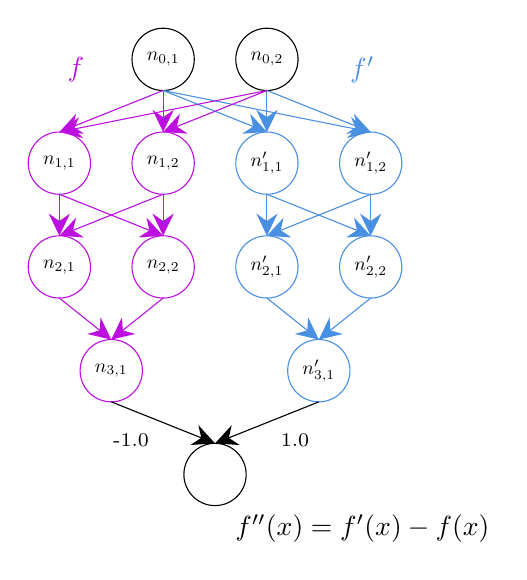
\begin{tikzpicture}[x=0.75pt,y=0.75pt,yscale=-1,xscale=1]
%uncomment if require: \path (0,319.46665954589844); %set diagram left start at 0, and has height of 319.46665954589844

%Shape: Circle [id:dp9204049738408316]
\draw   (160,45) .. controls (160,36.72) and (166.72,30) .. (175,30) .. controls (183.28,30) and (190,36.72) .. (190,45) .. controls (190,53.28) and (183.28,60) .. (175,60) .. controls (166.72,60) and (160,53.28) .. (160,45) -- cycle ;
%Shape: Circle [id:dp7103560225890297]
\draw   (210,45) .. controls (210,36.72) and (216.72,30) .. (225,30) .. controls (233.28,30) and (240,36.72) .. (240,45) .. controls (240,53.28) and (233.28,60) .. (225,60) .. controls (216.72,60) and (210,53.28) .. (210,45) -- cycle ;
%Shape: Circle [id:dp506809250809305]
\draw  [color={rgb, 255:red, 74; green, 144; blue, 226 }  ,draw opacity=1 ] (210,95) .. controls (210,86.72) and (216.72,80) .. (225,80) .. controls (233.28,80) and (240,86.72) .. (240,95) .. controls (240,103.28) and (233.28,110) .. (225,110) .. controls (216.72,110) and (210,103.28) .. (210,95) -- cycle ;
%Shape: Circle [id:dp884342585452375]
\draw  [color={rgb, 255:red, 74; green, 144; blue, 226 }  ,draw opacity=1 ] (260,95) .. controls (260,86.72) and (266.72,80) .. (275,80) .. controls (283.28,80) and (290,86.72) .. (290,95) .. controls (290,103.28) and (283.28,110) .. (275,110) .. controls (266.72,110) and (260,103.28) .. (260,95) -- cycle ;
%Shape: Circle [id:dp822908230674345]
\draw  [color={rgb, 255:red, 189; green, 16; blue, 224 }  ,draw opacity=1 ] (160,95) .. controls (160,86.72) and (166.72,80) .. (175,80) .. controls (183.28,80) and (190,86.72) .. (190,95) .. controls (190,103.28) and (183.28,110) .. (175,110) .. controls (166.72,110) and (160,103.28) .. (160,95) -- cycle ;
%Shape: Circle [id:dp8363894308909379]
\draw  [color={rgb, 255:red, 189; green, 16; blue, 224 }  ,draw opacity=1 ] (110,95) .. controls (110,86.72) and (116.72,80) .. (125,80) .. controls (133.28,80) and (140,86.72) .. (140,95) .. controls (140,103.28) and (133.28,110) .. (125,110) .. controls (116.72,110) and (110,103.28) .. (110,95) -- cycle ;
%Shape: Circle [id:dp8497915297699957]
\draw  [color={rgb, 255:red, 189; green, 16; blue, 224 }  ,draw opacity=1 ] (110,145) .. controls (110,136.72) and (116.72,130) .. (125,130) .. controls (133.28,130) and (140,136.72) .. (140,145) .. controls (140,153.28) and (133.28,160) .. (125,160) .. controls (116.72,160) and (110,153.28) .. (110,145) -- cycle ;
%Shape: Circle [id:dp4877577801962616]
\draw  [color={rgb, 255:red, 189; green, 16; blue, 224 }  ,draw opacity=1 ] (160,145) .. controls (160,136.72) and (166.72,130) .. (175,130) .. controls (183.28,130) and (190,136.72) .. (190,145) .. controls (190,153.28) and (183.28,160) .. (175,160) .. controls (166.72,160) and (160,153.28) .. (160,145) -- cycle ;
%Shape: Circle [id:dp4262388983828441]
\draw  [color={rgb, 255:red, 74; green, 144; blue, 226 }  ,draw opacity=1 ] (210,145) .. controls (210,136.72) and (216.72,130) .. (225,130) .. controls (233.28,130) and (240,136.72) .. (240,145) .. controls (240,153.28) and (233.28,160) .. (225,160) .. controls (216.72,160) and (210,153.28) .. (210,145) -- cycle ;
%Shape: Circle [id:dp6685783518531574]
\draw  [color={rgb, 255:red, 74; green, 144; blue, 226 }  ,draw opacity=1 ] (260,145) .. controls (260,136.72) and (266.72,130) .. (275,130) .. controls (283.28,130) and (290,136.72) .. (290,145) .. controls (290,153.28) and (283.28,160) .. (275,160) .. controls (266.72,160) and (260,153.28) .. (260,145) -- cycle ;
%Shape: Circle [id:dp44386673453797665]
\draw  [color={rgb, 255:red, 189; green, 16; blue, 224 }  ,draw opacity=1 ] (135,195) .. controls (135,186.72) and (141.72,180) .. (150,180) .. controls (158.28,180) and (165,186.72) .. (165,195) .. controls (165,203.28) and (158.28,210) .. (150,210) .. controls (141.72,210) and (135,203.28) .. (135,195) -- cycle ;
%Shape: Circle [id:dp5902710186002892]
\draw  [color={rgb, 255:red, 74; green, 144; blue, 226 }  ,draw opacity=1 ] (235,195) .. controls (235,186.72) and (241.72,180) .. (250,180) .. controls (258.28,180) and (265,186.72) .. (265,195) .. controls (265,203.28) and (258.28,210) .. (250,210) .. controls (241.72,210) and (235,203.28) .. (235,195) -- cycle ;
%Shape: Circle [id:dp11410611211945154]
\draw   (185,245) .. controls (185,236.72) and (191.72,230) .. (200,230) .. controls (208.28,230) and (215,236.72) .. (215,245) .. controls (215,253.28) and (208.28,260) .. (200,260) .. controls (191.72,260) and (185,253.28) .. (185,245) -- cycle ;
%Straight Lines [id:da3660185657298589]
\draw [color={rgb, 255:red, 189; green, 16; blue, 224 }  ,draw opacity=1 ]   (175,60) -- (175,78) ;
\draw [shift={(175,80)}, rotate = 270] [fill={rgb, 255:red, 189; green, 16; blue, 224 }  ,fill opacity=1 ][line width=0.75]  [draw opacity=0] (10.72,-5.15) -- (0,0) -- (10.72,5.15) -- (7.12,0) -- cycle    ;

%Straight Lines [id:da6340834663498455]
\draw [color={rgb, 255:red, 189; green, 16; blue, 224 }  ,draw opacity=1 ]   (175,60) -- (126.86,79.26) ;
\draw [shift={(125,80)}, rotate = 338.2] [fill={rgb, 255:red, 189; green, 16; blue, 224 }  ,fill opacity=1 ][line width=0.75]  [draw opacity=0] (10.72,-5.15) -- (0,0) -- (10.72,5.15) -- (7.12,0) -- cycle    ;

%Straight Lines [id:da62422960640828]
\draw [color={rgb, 255:red, 74; green, 144; blue, 226 }  ,draw opacity=1 ]   (175,60) -- (273.04,79.61) ;
\draw [shift={(275,80)}, rotate = 191.31] [fill={rgb, 255:red, 74; green, 144; blue, 226 }  ,fill opacity=1 ][line width=0.75]  [draw opacity=0] (10.72,-5.15) -- (0,0) -- (10.72,5.15) -- (7.12,0) -- cycle    ;

%Straight Lines [id:da7161221619909236]
\draw [color={rgb, 255:red, 74; green, 144; blue, 226 }  ,draw opacity=1 ]   (225,60) -- (225,78) ;
\draw [shift={(225,80)}, rotate = 270] [fill={rgb, 255:red, 74; green, 144; blue, 226 }  ,fill opacity=1 ][line width=0.75]  [draw opacity=0] (10.72,-5.15) -- (0,0) -- (10.72,5.15) -- (7.12,0) -- cycle    ;

%Straight Lines [id:da2931692798818335]
\draw [color={rgb, 255:red, 74; green, 144; blue, 226 }  ,draw opacity=1 ]   (175,60) -- (223.14,79.26) ;
\draw [shift={(225,80)}, rotate = 201.8] [fill={rgb, 255:red, 74; green, 144; blue, 226 }  ,fill opacity=1 ][line width=0.75]  [draw opacity=0] (10.72,-5.15) -- (0,0) -- (10.72,5.15) -- (7.12,0) -- cycle    ;

%Straight Lines [id:da7257821808480903]
\draw [color={rgb, 255:red, 74; green, 144; blue, 226 }  ,draw opacity=1 ]   (225,60) -- (273.14,79.26) ;
\draw [shift={(275,80)}, rotate = 201.8] [fill={rgb, 255:red, 74; green, 144; blue, 226 }  ,fill opacity=1 ][line width=0.75]  [draw opacity=0] (10.72,-5.15) -- (0,0) -- (10.72,5.15) -- (7.12,0) -- cycle    ;

%Straight Lines [id:da9549766786831592]
\draw [color={rgb, 255:red, 189; green, 16; blue, 224 }  ,draw opacity=1 ]   (225,60) -- (176.86,79.26) ;
\draw [shift={(175,80)}, rotate = 338.2] [fill={rgb, 255:red, 189; green, 16; blue, 224 }  ,fill opacity=1 ][line width=0.75]  [draw opacity=0] (10.72,-5.15) -- (0,0) -- (10.72,5.15) -- (7.12,0) -- cycle    ;

%Straight Lines [id:da7473462231383561]
\draw [color={rgb, 255:red, 189; green, 16; blue, 224 }  ,draw opacity=1 ]   (225,60) -- (126.96,79.61) ;
\draw [shift={(125,80)}, rotate = 348.69] [fill={rgb, 255:red, 189; green, 16; blue, 224 }  ,fill opacity=1 ][line width=0.75]  [draw opacity=0] (10.72,-5.15) -- (0,0) -- (10.72,5.15) -- (7.12,0) -- cycle    ;

%Straight Lines [id:da6347150163020211]
\draw [color={rgb, 255:red, 189; green, 16; blue, 224 }  ,draw opacity=1 ]   (175,110) -- (175,128) ;
\draw [shift={(175,130)}, rotate = 270] [fill={rgb, 255:red, 189; green, 16; blue, 224 }  ,fill opacity=1 ][line width=0.75]  [draw opacity=0] (10.72,-5.15) -- (0,0) -- (10.72,5.15) -- (7.12,0) -- cycle    ;

%Straight Lines [id:da33585563428931897]
\draw [color={rgb, 255:red, 189; green, 16; blue, 224 }  ,draw opacity=1 ]   (175,110) -- (126.86,129.26) ;
\draw [shift={(125,130)}, rotate = 338.2] [fill={rgb, 255:red, 189; green, 16; blue, 224 }  ,fill opacity=1 ][line width=0.75]  [draw opacity=0] (10.72,-5.15) -- (0,0) -- (10.72,5.15) -- (7.12,0) -- cycle    ;

%Straight Lines [id:da6150681893695612]
\draw [color={rgb, 255:red, 189; green, 16; blue, 224 }  ,draw opacity=1 ]   (125,110) -- (125,128) ;
\draw [shift={(125,130)}, rotate = 270] [fill={rgb, 255:red, 189; green, 16; blue, 224 }  ,fill opacity=1 ][line width=0.75]  [draw opacity=0] (10.72,-5.15) -- (0,0) -- (10.72,5.15) -- (7.12,0) -- cycle    ;

%Straight Lines [id:da24917677142291106]
\draw [color={rgb, 255:red, 189; green, 16; blue, 224 }  ,draw opacity=1 ]   (125,110) -- (173.14,129.26) ;
\draw [shift={(175,130)}, rotate = 201.8] [fill={rgb, 255:red, 189; green, 16; blue, 224 }  ,fill opacity=1 ][line width=0.75]  [draw opacity=0] (10.72,-5.15) -- (0,0) -- (10.72,5.15) -- (7.12,0) -- cycle    ;

%Straight Lines [id:da16536032590300243]
\draw [color={rgb, 255:red, 189; green, 16; blue, 224 }  ,draw opacity=1 ]   (125,160) -- (148.44,178.75) ;
\draw [shift={(150,180)}, rotate = 218.66] [fill={rgb, 255:red, 189; green, 16; blue, 224 }  ,fill opacity=1 ][line width=0.75]  [draw opacity=0] (10.72,-5.15) -- (0,0) -- (10.72,5.15) -- (7.12,0) -- cycle    ;

%Straight Lines [id:da06800155466556901]
\draw [color={rgb, 255:red, 189; green, 16; blue, 224 }  ,draw opacity=1 ]   (175,160) -- (151.56,178.75) ;
\draw [shift={(150,180)}, rotate = 321.34000000000003] [fill={rgb, 255:red, 189; green, 16; blue, 224 }  ,fill opacity=1 ][line width=0.75]  [draw opacity=0] (10.72,-5.15) -- (0,0) -- (10.72,5.15) -- (7.12,0) -- cycle    ;

%Straight Lines [id:da4955822084224828]
\draw    (150,210) -- (198.14,229.26) ;
\draw [shift={(200,230)}, rotate = 201.8] [fill={rgb, 255:red, 0; green, 0; blue, 0 }  ][line width=0.75]  [draw opacity=0] (10.72,-5.15) -- (0,0) -- (10.72,5.15) -- (7.12,0) -- cycle    ;

%Straight Lines [id:da3383340031428528]
\draw    (250,210) -- (201.86,229.26) ;
\draw [shift={(200,230)}, rotate = 338.2] [fill={rgb, 255:red, 0; green, 0; blue, 0 }  ][line width=0.75]  [draw opacity=0] (10.72,-5.15) -- (0,0) -- (10.72,5.15) -- (7.12,0) -- cycle    ;

%Straight Lines [id:da09011875495468658]
\draw [color={rgb, 255:red, 74; green, 144; blue, 226 }  ,draw opacity=1 ]   (225,160) -- (248.44,178.75) ;
\draw [shift={(250,180)}, rotate = 218.66] [fill={rgb, 255:red, 74; green, 144; blue, 226 }  ,fill opacity=1 ][line width=0.75]  [draw opacity=0] (10.72,-5.15) -- (0,0) -- (10.72,5.15) -- (7.12,0) -- cycle    ;

%Straight Lines [id:da22312300392620754]
\draw [color={rgb, 255:red, 74; green, 144; blue, 226 }  ,draw opacity=1 ]   (275,160) -- (251.56,178.75) ;
\draw [shift={(250,180)}, rotate = 321.34000000000003] [fill={rgb, 255:red, 74; green, 144; blue, 226 }  ,fill opacity=1 ][line width=0.75]  [draw opacity=0] (10.72,-5.15) -- (0,0) -- (10.72,5.15) -- (7.12,0) -- cycle    ;

%Straight Lines [id:da8357798363095627]
\draw [color={rgb, 255:red, 74; green, 144; blue, 226 }  ,draw opacity=1 ]   (275,110) -- (275,128) ;
\draw [shift={(275,130)}, rotate = 270] [fill={rgb, 255:red, 74; green, 144; blue, 226 }  ,fill opacity=1 ][line width=0.75]  [draw opacity=0] (10.72,-5.15) -- (0,0) -- (10.72,5.15) -- (7.12,0) -- cycle    ;

%Straight Lines [id:da13412901969707558]
\draw [color={rgb, 255:red, 74; green, 144; blue, 226 }  ,draw opacity=1 ]   (225,110) -- (225,128) ;
\draw [shift={(225,130)}, rotate = 270] [fill={rgb, 255:red, 74; green, 144; blue, 226 }  ,fill opacity=1 ][line width=0.75]  [draw opacity=0] (10.72,-5.15) -- (0,0) -- (10.72,5.15) -- (7.12,0) -- cycle    ;

%Straight Lines [id:da5973635189469982]
\draw [color={rgb, 255:red, 74; green, 144; blue, 226 }  ,draw opacity=1 ]   (225,110) -- (273.14,129.26) ;
\draw [shift={(275,130)}, rotate = 201.8] [fill={rgb, 255:red, 74; green, 144; blue, 226 }  ,fill opacity=1 ][line width=0.75]  [draw opacity=0] (10.72,-5.15) -- (0,0) -- (10.72,5.15) -- (7.12,0) -- cycle    ;

%Straight Lines [id:da6136321172381055]
\draw [color={rgb, 255:red, 74; green, 144; blue, 226 }  ,draw opacity=1 ]   (275,110) -- (226.86,129.26) ;
\draw [shift={(225,130)}, rotate = 338.2] [fill={rgb, 255:red, 74; green, 144; blue, 226 }  ,fill opacity=1 ][line width=0.75]  [draw opacity=0] (10.72,-5.15) -- (0,0) -- (10.72,5.15) -- (7.12,0) -- cycle    ;


% Text Node
\draw (159.5,228.5) node  [align=left] {{\scriptsize -1.0}};
% Text Node
\draw (238.5,228.5) node  [align=left] {{\scriptsize 1.0}};
% Text Node
%\draw (200,245) node   {$n $};
\draw (271,271) node   {$f''(x) = f'(x) - f(x) $};
% Text Node
\draw (175,95) node [scale=0.7]  {$n_{1,2}$};
% Text Node
\draw (125,95) node [scale=0.7]  {$n_{1,1}$};
% Text Node
\draw (225,95) node [scale=0.7]  {$n'_{1,1}$};
% Text Node
\draw (275,95) node [scale=0.7]  {$n'_{1,2}$};
% Text Node
\draw (275,145) node [scale=0.7]  {$n'_{2,2}$};
% Text Node
\draw (225,145) node [scale=0.7]  {$n'_{2,1}$};
% Text Node
\draw (250,195) node [scale=0.7]  {$n'_{3,1}$};
% Text Node
\draw (150,195) node [scale=0.7]  {$n_{3,1}$};
% Text Node
\draw (125,145) node [scale=0.7]  {$n_{2,1}$};
% Text Node
\draw (175,145) node [scale=0.7]  {$n_{2,2}$};
% Text Node
\draw (175,45) node [scale=0.7]  {$n_{0,1}$};
% Text Node
\draw (225,45) node [scale=0.7]  {$n_{0,2}$};
% Text Node
\draw (133,50) node   {\color{rgb, 255:red, 189; green, 16; blue, 224} $f$};
% Text Node
\draw (271,50) node   {\color{rgb, 255:red, 74; green, 144; blue, 226 } $f'$};


\end{tikzpicture}

}
	\caption{Composition approach for proving equivalence of $ f(x) $ and $ f'(x)
	$.}
	\label{fig:subbed_nnets_intro}
\end{figure}

\section{Limitations of Current Verification Tools}
We first layout in more detail the limitations of current verification tools
because these lead to insights for how to address them. As previously mentioned,
current tools are neither accurate nor general for proving equivalence (or differential
properties in general). Here, we highlight \textit{why} this is the case.

Current tools are not accurate proving equivalence because they do not have the
ability to exploit the structural similarities of two closely related
networks. They work by computing an
over-approximation on the values of each neuron in a neural network in a forward
layer-by-layer fashion. While the approximations computed for the neurons in the
early layers are relatively accurate, the approximations become overly
conservative in the later layers as the neural network's behavior becomes
increasingly complex. Using the composition
approach illustrated in Figure~\ref{fig:subbed_nnets_intro}, these tools would
compute an
over-approximation of $ f(x) $ and $ f'(x) $  \textit{independently}, and then
subtract them to approximate the difference of the two networks over all inputs.
However, as previously mentioned, these approximations for $ f(x) $ and $ f'(x) $ will
be overly
conservative for deeper networks, and thus the resulting approximation on the
difference will be too conservative to verify reasonable equivalence properties.
We empirically demonstrate this in Chapter~\ref{ch:reludiff}.

In addition, current tools are not general because they require an expert to
hand-craft a \textit{linear approximation} for the neural network's activation
functions in order to accurately over-approximate the values of a given neuron.
While there exist techniques to compute linear approximations for arbitrary
functions without the need for an expert, such as the techniques used in rigorous global
optimization~\cite{chabert2009contractor,trombettoni2011inner} and nonlinear
constraint solving~\cite{gao2013dreal}, we
show that these approaches produce overly-conservative approximations. This
results in poor accuracy, and thus current tools are not general. We
empirically demonstrate this poor accuracy in Chapters~\ref{ch:onlinesyn}
and~\ref{ch:offlinesyn}.


\section{Hypotheses and Insights}
Based on these limitations, we propose three testable hypotheses to improve the
accuracy and generality of existing tools for differential properties, and we
present insights that inspired these hypotheses. We begin with hypotheses and
insights for improving the accuracy.

\begin{table}[h]
	\centering
	\large
	\begin{tabular}{|p{0.2\linewidth}|p{0.7\linewidth}|} \hline
		\textbf{Hypothesis 1a}      &
		Approximating the difference layer-by-layer can significantly improve
		accuracy versus existing tools for differential properties. \\ \hline
		\textbf{Insight 1a}        &
		This approach begins approximating the difference \textit{before}
		significant approximation errors accumulate. \\ \hline
%		\textbf{Hypothesis 1b}        &
%		Symbolic approximations can further improve the accuracy of the
%		layer-by-layer approximation. \\ \hline
%		\textbf{Insight 1b}        &
%		Symbols capture dependency information, allowing terms to
%		``cancel,'' and thus reducing approximation errors. \\ \hline
	\end{tabular}
\end{table}

Hypothesis 1a suggests a new technique for approximating the difference between
two structurally similar neural networks. Prior work independently computes
approximations for the output neurons, e.g. $ n_{3,1} $ and $ n'_{3,1} $ in
Figure~\ref{fig:subbed_nnets_intro}, and then subtracts them to approximate the
difference. In our
new technique, we first approximate the difference between the neurons of the
first layers, e.g. we compute an approximation for $ n'_{1,1} - n_{1,1} $ and $
n'_{1,2} - n_{1,2} $. Then we use this result to approximate $ n'_{2,1} - n_{2,1}
$ and $ n'_{2,2} - n_{2,2} $, and repeat until the final output layer. Our
intuition is laid out in Insight 1a.

\begin{table}[h]
	\centering
	\large
	\begin{tabular}{|p{0.2\linewidth}|p{0.7\linewidth}|} \hline
%		\textbf{Hypothesis 1a}      &
%		Approximating the difference layer-by-layer can significantly improve
%		accuracy versus existing tools for differential properties. \\ \hline
%		\textbf{Insight 1a}        &
%		This approach begins approximating the difference \textit{before}
%		significant approximation errors accumulate. \\ \hline
		\textbf{Hypothesis 1b}        &
		Symbolic approximations can further improve the accuracy of the
		layer-by-layer approximation. \\ \hline
		\textbf{Insight 1b}        &
		Symbols capture dependency information, allowing terms to
		``cancel,'' and thus reducing approximation errors. \\ \hline
	\end{tabular}
\end{table}

Hypothesis 1b suggests a technique for improving the accuracy of the technique
laid out by Hypothesis 1a. Our intuition, described in Insight 1b, is inspired by
program verification techniques such as symbolic
execution~\cite{king1976symbolic} and abstract interpretation~\cite{CousotC77},
which use symbols to represent inputs, resulting in more accurate approximations.
%A prerequisite for symbolic approximations are linear approximations of the
%neural network's activation functions, thus we develop novel linear
%approximations for over-approximating the difference between two neurons of two
%different networks (e.g. $ n_{2,1} - n'_{2,1} $).

Our final hypothesis and insight aim to improve the generality of existing tools.
As previously mentioned, the key challenge to obtaining accurate approximations
lies in computing linear approximations for the neural network's activation
functions. Prior to our work, an expert needed to hand-craft these linear
approximations in order to be accurate, which poses significant limitations on
the generality of existing verification tools. Thus we propose the following hypothesis.

\begin{table}[h]
	\centering
	\large
	\begin{tabular}{|p{0.2\linewidth}|p{0.7\linewidth}|} \hline
		\textbf{Hypothesis 2}      &
		Automatically synthesizing linear approximations for the activation
		functions can significantly improve accuracy for general activation
		functions. \\ \hline
		\textbf{Insight 2}        &
		Both our work and prior work demonstrated significant accuracy
		improvements. \\ \hline
	\end{tabular}
\end{table}

This hypothesis and insight follow naturally based off the results from prior
work, which demonstrated that linear approximations of the neural network's
activation functions are vital for accuracy.
%To test this hypothesis, we propose
%two novel techniques for automatically synthesizing linear approximations
%(without  the need for an expert's input), and compare their accuracy with the
%best alternative technique.

\section{Contributions}
This dissertation tests the above hypotheses by proposing and evaluating four
novel techniques
for \textit{accurate} and \textit{general} differential verification of deep
neural networks. The first two techniques implement the ideas suggested by
Hypotheses 1a and 1b, which aim to improve the accuracy when approximating the
difference between two networks. These techniques focus specifically on
feed-forward ReLU networks. The third and fourth techniques implement the idea
suggested by Hypothesis 2, which aims to improve the accuracy of approximations
for non-standard neural networks. For each technique, we compare with the best
alternative technique to test our hypotheses. Below we summarize the techniques
and results, which make up the core contribution of this dissertation.

\subsection{Approximating the Difference Layer-by-Layer}
The first technique that we propose improves the accuracy when approximating the
difference between two structurally similar neural networks by approximating
their difference layer-by-layer. To implement such a technique, we make two key
intellectual contributions. First, we formally derive equations that relate the
intermediate computations of the two neural networks, thus allowing the
layer-by-layer approximation. We then use \textit{interval analysis} to
rigorously bound these
equations, resulting in an over-approximation on the difference between the two
networks. Second, we develop a novel refinement technique, which can
iteratively improve the accuracy of the computed approximation. We
design the technique for ReLU networks, and we compare with two state-of-the-art
(single network) verification tools. We demonstrate one to two
orders-of-magnitude improvement in both accuracy of the approximations, and
runtime to prove/disprove equivalence properties, thus confirming Hypothesis 1a.

\subsection{Symbolic Approximations for the Difference}
The second technique that we propose further improves the accuracy of the
layer-by-layer approximation by using symbolic approximations. To implement this
technique, we make two more intellectual contributions. First, we develop a novel
linear approximation for the difference between two neurons, which allows us to
maintain symbols in the intervals. Second, we propose a technique to
judiciously create new symbolic variables that represent the intermediate neurons
of the two networks. We compare this symbolic approach with our first technique
and demonstrate further improvements in both accuracy and runtime, thus
confirming Hypothesis 1b.

\subsection{Online Synthesis of Linear Approximations}
The third technique that we propose improves the accuracy of approximations for
neural networks with non-standard activation functions (thus improving
generality) by automatically synthesizing linear approximations. To implement
this technique, we develop a novel approach that combines efficient (unsound) heuristics
with a nonlinear SMT solver to guarantee soundness. We call this technique
\textit{online}
because we directly call SMT solvers to synthesize the linear approximations. We compare
our synthesis approach with hand-crafted approximations, and demonstrate significant
improvements in accuracy, thus confirming Hypothesis 2.

\subsection{Offline Synthesis of Linear Approximations}
A key limitation of the third technique is its online nature. The use of solvers
incurs a significant runtime overhead when attempting to prove a given property. The
final technique that we propose again improves generality, but
alleviates the runtime overhead by performing the synthesis \textit{offline}.
Whereas the third technique directly uses the SMT solver to compute the linear
approximation, this technique synthesizes a \textit{static imperative program}
that computes linear approximations. Since the synthesized program does not call
expensive solvers, it computes linear approximations several orders of magnitude
faster than the online synthesis technique. While faster, the offline approach is
not nearly as accurate as the online approach. However, the offline approach is
still significantly more accurate than hand-crafted approximations, thus again
confirming Hypothesis 2.

\section{Overview}
This dissertation is organized as follows. In Chapter~\ref{ch:background}, we
discuss the most closely related work to ours, and how our work differs. The next
four chapters present the main contributions of this dissertation.
Chapter~\ref{ch:reludiff} presents our new technique for approximating the
difference between two neural network in a layer-by-layer fashion, which has been
published~\cite{paulsen2020reludiff} in the main track of the IEEE/ACM
International Conference on Software Engineering. Chapter~\ref{ch:neurodiff}
presents our symbolic technique for the layer-by-layer approximation, and has been
published~\cite{paulsen2020neurodiff} in the main track of the IEEE/ACM
International Conference on Automated Software Engineering.
Chapter~\ref{ch:onlinesyn} presents our online technique for synthesizing linear
approximations, and has been published~\cite{paulsen2022linsyn} in the main track
of the International Conference on Tools and Algorithms for the Construction and
Analysis of Systems. Chapter~\ref{ch:offlinesyn} presents our offline technique
for synthesizing linear approximations, and has been published at the
International Conference on Computer Aided Verification.
Finally, in Chapter~\ref{ch:conclusions} we summarize the contributions of this
dissertation, and present potential directions for future work.
